\textbf{Kolvpump}\\
Första modellen är en kolvpump som pumpar ingredienserna med hjälp av en kolv som rör sig fram och tillbaka i en cylinder. Pumpen är utformad för att hantera vätskor, halvfasta och trögflytande produkter och den häller ingredienserna på degen med hjälp av ett munstycke. Doseringsvolymen på matrialet kan bestämmas genom att helt enkelt öka eller minska kolvens rörelse. Figuren~\ref{kolvpump} visar example på en kolvpump.

Födelar med pumptekniken:
\begin{itemize}
	\item Påfyllningsvolymen är exakt doserad för att minska slöseriet.
	\item Fördelningen av olika produkter och halvfasta ämnen i samma behållare är korrekt repeterbar.
	\item Pumptekniken mäter ingredienserna med precision, tack vare servodrivenkolv.
	\item Pumpen kan rengöras på plats utan nedmontering.
\end{itemize}

\begin{figure}[h]
	\begin{center}
		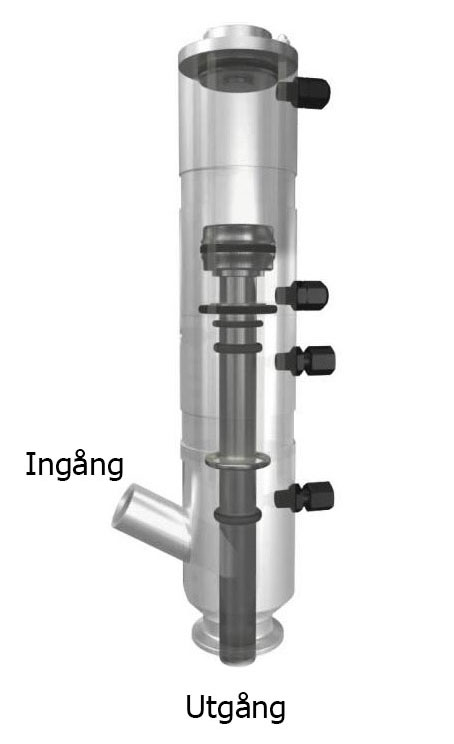
\includegraphics[scale=0.5]{images/maxresdefault.jpg}
		\caption{Kolvpump med exakt dosering för fyllningsmaterial~\cite{Dosering pump}}
		\label{kolvpump}	
	\end{center}
\end{figure}

\newpage
\textbf{Kugghjulspump}\\*
Figuren ~\ref{kugghjulpump} visar en kugghjulspump som består av två kugghjul, ett drivande kugghjul och ett drivet kugghjul.  Materialet följer luckorna mellan kuggarna genom pumpen. Kugghjulspumpar lämpar sig bäst för höga pumphöjder(vertikala sträcka mellan slutväxel och pump)\cite{kugghjul pump}.

Pumpen används allmänt i moderna hydrauliska system på grund av höga prestanda och lång livslängd.

\begin{figure}[h]
	\begin{center}
		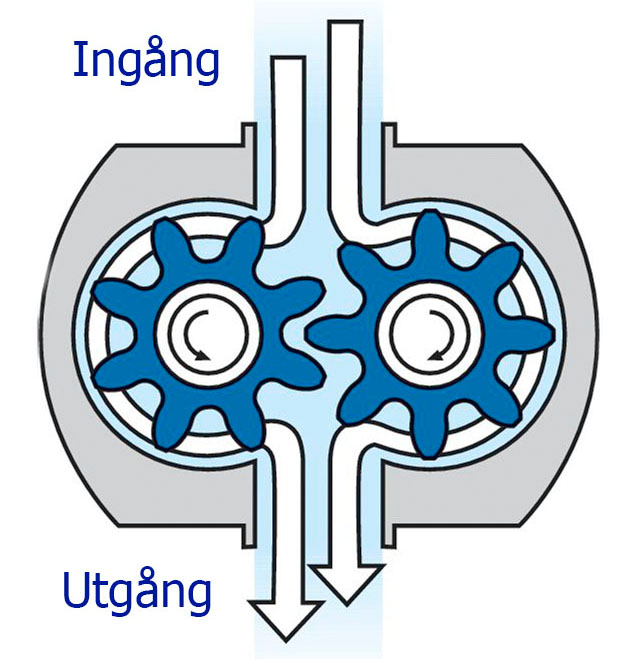
\includegraphics[scale=0.25]{images/68637(1).jpg}
		\caption{Kugghjulspump, ett av hjulen drivs av den andra}
		\label{kugghjulpump}	
	\end{center}
\end{figure}